\documentclass[10pt]{article}

%%%%    FORMATTING    %%%%
\usepackage{url}
\usepackage[utf8]{inputenc}
\usepackage{amsmath}
\usepackage{amssymb}
%\usepackage{wasysym}
\usepackage[dvipsnames]{xcolor}
\usepackage[version=4]{mhchem}
\usepackage{verbatim}
\usepackage{graphicx}
\usepackage[export]{adjustbox}
\usepackage[margin=1in]{geometry}
\usepackage[titletoc, title]{appendix}
\usepackage{hyperref}
\hypersetup{
    colorlinks = true,
    citecolor = red,
    linkcolor = blue,
    urlcolor = black,
}
%For code in appendix
\usepackage{listings}
\usepackage{color}
\definecolor{mygreen}{rgb}{0,0.6,0}
\definecolor{mygray}{rgb}{0.5,0.5,0.5}
\definecolor{mymauve}{rgb}{0.58,0,0.82}
\lstset{ %
  backgroundcolor=\color{white},   % choose the background color
  basicstyle=\footnotesize,        % size of fonts used for the code
  breaklines=true,                 % automatic line breaking only at whitespace
  captionpos=b,                    % sets the caption-position to bottom
  commentstyle=\color{mygreen},    % comment style
  escapeinside={\%*}{*)},          % if you want to add LaTeX within your code
  keywordstyle=\color{blue},       % keyword style
  stringstyle=\color{mymauve},     % string literal style
  frame = tb,
  numbers = left
}




\title{nEXO OD FLUKA Simulations Manual}
\author{Regan Ross}

%%%%    BEGIN DOCUMENT    %%%
\begin{document}

%%%%    Title Page    %%%
\begin{titlepage}
    \maketitle
    \vspace{4cm}
    \centering
    % \includegraphics*[scale=0.5, frame]{./figs/muons_det.png}
\end{titlepage}

\begin{abstract}
    This document is intented to provide insight into the functioning of the nEXO FLUKA simulations and justifications for choices made in their design. Further, this work should provide a near comprehensive baseline for anyone willing to replicate similar cosmogenic studies for the nEXO collaboration, or even another. FLUKA can be a daunting software to work with given it is written in FORTRAN77, has sparse documentation, and whose source code, without a specific licence, is veiled to the user. However, this proprietary simulation program is fast and rich with built-in features that have been used extensively for decades. Moreover, it is particularly useful for the case of studying cosmogenic muons at several hundred GeV energies and their secondaries. This document will provide an overview and explanation of the FLUKA features enabled for the specific nEXO Outer Detector (OD) case and an overview of the additional user routines, scripts, and containerization procedures that are all ancilliary to the base simulations (but required to run the simulations on the SDF cluster and perform the more in-depth analyses required by our questions).
\end{abstract}


\vspace{1.5cm}
\listoffigures

\newpage
\tableofcontents

\break
%%%%%%%%%%%%%%%%%%%%%%%%%%%%%%%%%%%%%%
%                                   %
%%%%    The FLUKA Input File     %%%%
%                                   %
%%%%%%%%%%%%%%%%%%%%%%%%%%%%%%%%%%%%%%
\part*{The FLUKA Input File (`.inp')}
\section{Introduction}
    \paragraph{}
    The input file is exactly as it is named— it is the De facto interface between the user and the FLUKA binaries. It contains, among other things, the entire physical configuration of the media through which the particles are transported, the defining characteristics of the impinging beam, options for enabling particular physical processes, definitions of materials, and cards to deploy default FLUKA scoring methods. It is a human-readable ascii file with a very specific format. Each input card in the input file must not contain more than 8 fields each of which has a character limit. This is due (presumably) to constraints in the early development of FLUKA. Programmed in FORTRAN77 which imposes constrains on the length of statements which, in the early days, were written into computers (with very little memory) using paper punch cards. Now, this formatting is an annoying anachronism but it probably does still keep the program slim and fast. Generally though, a user need not worry about writing the input file directly, as there is a great GUI interface to FLUKA called \textit{flair} which, by the way, is open source and contains all the possible input options. The next section will overview the specific components of the nEXO OD input file and the functions they serve.


\section{The nEXO OD Input File}

\subsection{Geometry}
\paragraph{}
Arguably the most important parts of the input file are the cards defining the configuration space— namely the detector and media with respect to the cartesian coordinate system. In FLUKA this is known as the \textit{geometry}. The geometry section of the input card is demarcated by \textbf{GEOBEGIN} and \textbf{GEOEND} cards. Between these two cards are first, cards for various \textit{bodies} which are basic 2D and 3D geometric surfaces and second, cards for \textit{regions} whose bounds are defined by combinations of geometric \textit{bodies}. For instance, a triplet of bodies could be a cylinder whose axis lies on the $z$-axis, and two planes lying parallel the $x-y$ plane at different $z$s. A region defined by these bodies could be the 3D cylindrical volume made by the cylinder body capped off on either end by the two planes. This is exactly the type of region representing the nEXO OD and the nEXO TPC. 

\begin{figure}[h]
    \begin{center}
    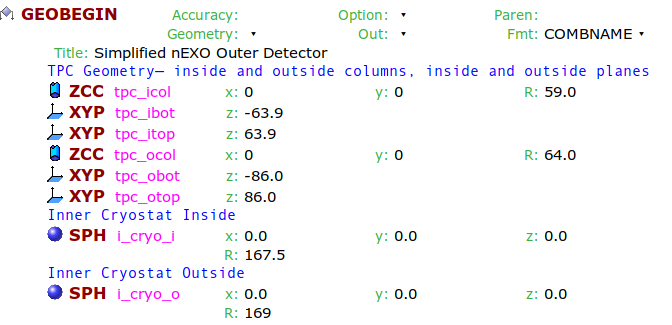
\includegraphics[scale=0.5]{geometry_1.png}
    \caption{An example of the geometry declarations in the input file}
    \label{fig:geometry1}
    \end{center}
\end{figure}

\paragraph{}
Figure \ref{fig:geometry1} shows the first part of the geometry declarations in the nEXO input file. We see the first card is the \textbf{GEOBEGIN} with the argument \textit{fmt} set to COMBNAME. This tells the FLUKA binaries how to read in the following geometry cards. This is not particularly important. This seems to be the default mode. Text in \textcolor{blue}{blue} indicates a comment (equivalent to a FORTRAN77 comment in the input file) and body variable names are in \textcolor{magenta}{pink} and are limited to lengths of 8 characters. The names or types of cards are fully capitalized and in \textcolor{Maroon}{maroon}. The argument names for each card are written in \textcolor{ForestGreen}{green} and the arguments follow with an 8 character length limit. These colour conventions hold for every other type of input card.

\part*{The Muon Source User Routine}

\part*{The Scoring User Routine (`mgdraw.f')}

\part*{Containerization with Singularity}

\part*{Interpreting Output}

% \clearpage
% % \appendixheaderon
% % \appendixpage
% % \begin{appendices}
    

% % \end{appendices}


% \newpage

% \section*{Acknowledgements}
% \paragraph{}


% \bibliographystyle{aip}
% \bibliography{manual.bib}

\end{document}